\begin{center}
	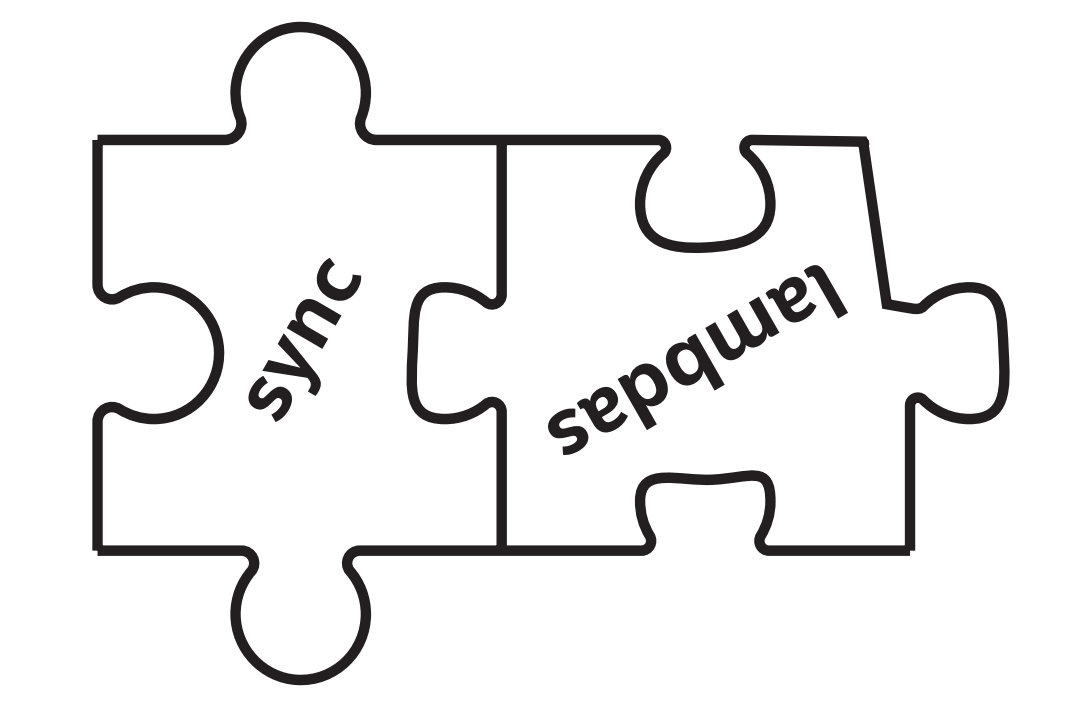
\includegraphics[width=0.5\textwidth]{content/chapter-10/images/1}
\end{center}

Thus far in this book, our code examples have represented kernels using C++ lambda expressions. Lambda expressions are a concise and convenient way to represent a kernel right where it is used, but they are not the only way to represent a kernel in SYCL. In this chapter, we will explore various ways to define kernels in detail, helping us to choose a kernel form that is most natural for our C++ coding needs.\par

This chapter explains and compares three ways to represent a kernel:\par

\begin{itemize}
	\item Lambda expressions
	\item Named function objects (functors)
	\item Interoperability with kernels created via other languages or APIs
\end{itemize}

This chapter closes with a discussion of how to explicitly manipulate kernels in a program object to control when and how kernels are compiled.\par




